\chapter{Environments examples}
\label{ch:environments}

\section{engineeringThesis.sty environments}

\begin{definition}
This is an example of a definition
\end{definition}

\begin{example}
This is an example of an example :)
\end{example}

\begin{proposition}
This is an example of a proposition.
\end{proposition}

\begin{lemma}
This is an example of a lemma.
\end{lemma}

\begin{corollary}
This is an example of a corollary
\end{corollary}

\begin{theorem}
This is an example of a theorem.
\end{theorem}

\begin{proof}
This is an example of a proof.
\end{proof}

\section{\LaTeX{} environments}

Table \ref{tab:ResistanceTable} is an example of both, how to create tables in \LaTeX{} and how to use cross-referencing. Equation \ref{eq:Schr} show the Schr\"{o}dinger equation, an example of how to write equations, and how to cross-reference equations \cite{Quantum}.

\begin{table}[h!]
	\centering
	\begin{tabular}{c | c}
		I & $\Omega$ \\ \hline
		12 & 4 \\
		10 & 6 \\
		8 & 8 \\
		6 & 10 \\
	\end{tabular}
	\caption[short caption]{long caption}% short caption is optional and if filled is used in the table of contents.
	\label{tab:ResistanceTable}
\end{table}

\begin{equation}
i\hbar \frac{\partial \psi}{\partial t} = -\frac{\hbar^2}{2m}\nabla^2 \psi + V(\mathbf{r})
\label{eq:Schr}
\end{equation}

Figure \ref{fig:WordVsLatex} show how to insert graphics in a \LaTeX{} documents and also how to cross-reference it.

\begin{figure}[h!]
\centering
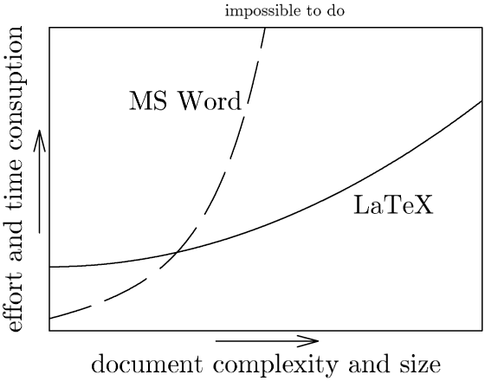
\includegraphics[width=0.6\textwidth]{images/WordVsLatex.png}
\caption{A plot show how much easier it is to write documents with \LaTeX{}} \label{fig:WordVsLatex}
\end{figure}